\section{Combinatorial Analysis}
\subsection{Subsets}

\begin{question}
    Let $\Omega$ be finite and $|\Omega| = n$. How many ways to \emph{partition} $\Omega$ into $k$ disjoint subsets $\Omega_1, \dots, \Omega_k$ with $|\Omega_i| = n_i$ (with $\sum_{i=1}^{k} n_i = n$)?
\end{question} 

\begin{answer} ~\vspace*{-1.5\baselineskip}
    \begin{align*}
        M &= \underset{\substack{\text{Choose} \\ \text{first part}}}{\binom{n}{n_1}} \underset{\substack{\text{Then choose} \\ \text{second part}}}{\binom{n - n_1}{n_2}} \binom{n - n_1 - n_2}{n_3} \dots \underbrace{\binom{n - (n_1 + \dots + n_{k - 1})}{n_k}}_{= 1} \\
        &= \frac{n!}{n_1! \cancel{(n - n_1)!}} \times \frac{\cancel{(n - n_1)!}}{n_2! \cancel{(n - n_1 - n_2)!}} \times \frac{\cancel{[n - (n + n_1 + \dots + n_{k - 1})]!}}{0! n_k!} \\
        &= \frac{n!}{n_1! n_2! \dots n_k!} \\
        &= \underbrace{\binom{n}{n_1, n_2, \dots, n_k}}_{\text{Multinomial coefficient}}
    \end{align*} 
    \emph{Key sanity check}

    - Does ordering of the subsets matter?

    E.g. Is $\Omega_2 = \{3, 4, 7\}, \Omega_3 = \{1, 5, 8\}$ equal to $\Omega_3 = \{3, 4, 7\}, \Omega_2 = \{1, 5, 8\}$? 
    No, ordering does matter as we put elements first in the second subset then the third.
\end{answer} 

\subsection{Random Walks}

\begin{figure}[h] 
    \centering 
    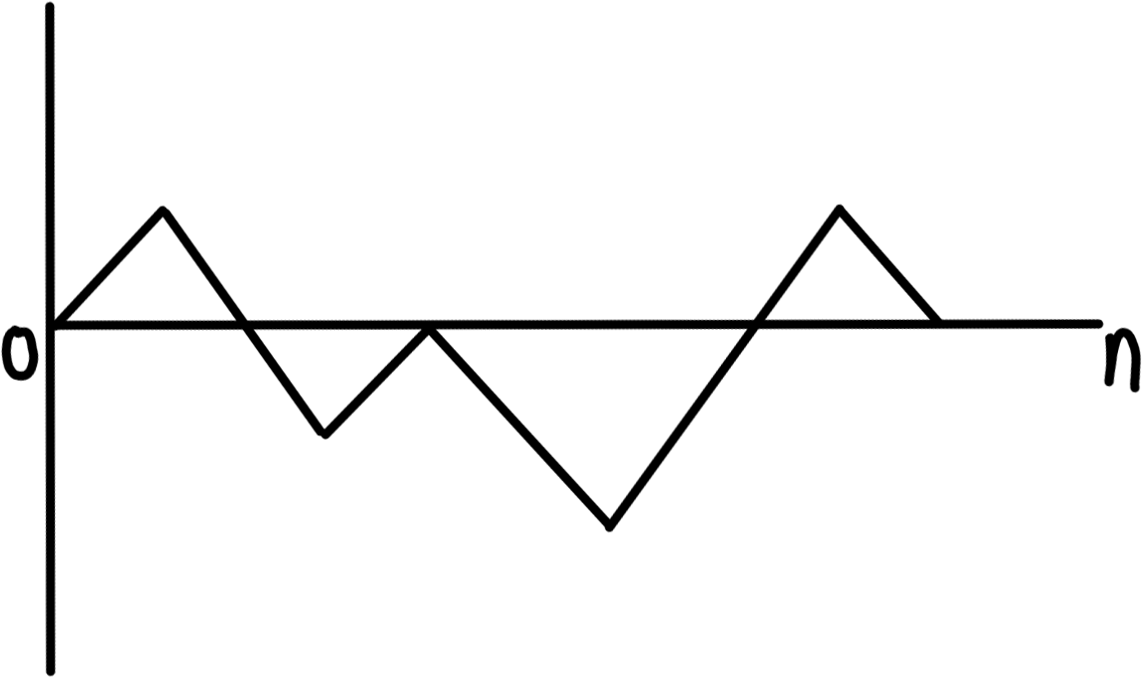
\includegraphics[height=5cm]{03-random} 
\end{figure}

\begin{gather*}
    \Omega = \{(X_0, X_1, \dots, X_n) : X_0 = 0, |X_n - X_{k - 1}| = 1 \ \forall \; k = 1, \dots, n\}. \\
    |\Omega| = 2^n \ \text{(we can go either up or down at each $k$)} \\
    \mathbb{P}(X_n = n) = \frac{1}{2^n} \\
    \mathbb{P}(X_n = 0) = 0 \text{ if $n$ is odd} \\
    \text{What about } \mathbb{P}(X_n = 0) \text{ when $n$ is even}
\end{gather*} 
\emph{Idea} - Choose $\frac{n}{2}$ $k$s for $X_k = X_{k - 1} + 1$ and the rest $X_k = X_{k-1} - 1$ (i.e. go up half the time and down the other half).
\begin{align*}
    \mathbb{P}(X_n = 0) &= 2^{-n} \binom{n}{\frac{n}{2}} \\
    &= \frac{n!}{2^n \left(\frac{n}{2}! \right)^2}
\end{align*} 

\begin{question}
    What happens when $n$ is large?
\end{question} 

\subsection{Stirling's Formula}

\begin{notation}
    Let $(a_n), (b_n)$ be two sequences.
    Say $a_n \sim b_n$ as $n \to \infty$ if $\frac{a_n}{b_n} \to 1$ as $n \to \infty$.
\end{notation} 

\begin{example}
    $n^2 + 5n + \frac{6}{n} \sim n^2$
\end{example} 

\begin{example}[Non-Example]
    $\exp \left( n^2 + 5n + \frac{6}{n} \right) \nsim \exp(n^2)$
\end{example} 

\begin{theorem}[Stirling]
    $n! \sim \sqrt{2 \pi} n^{n + \frac{1}{2}} e^{-n}$ as $n \to \infty$.
\end{theorem} 

\begin{theorem}[Weaker Version]
    $\log n! \sim n \log n$.
\end{theorem} 

\begin{proof}
    $\log(n!) = \log 2 + \dots + \log n$.
    {\par \centering 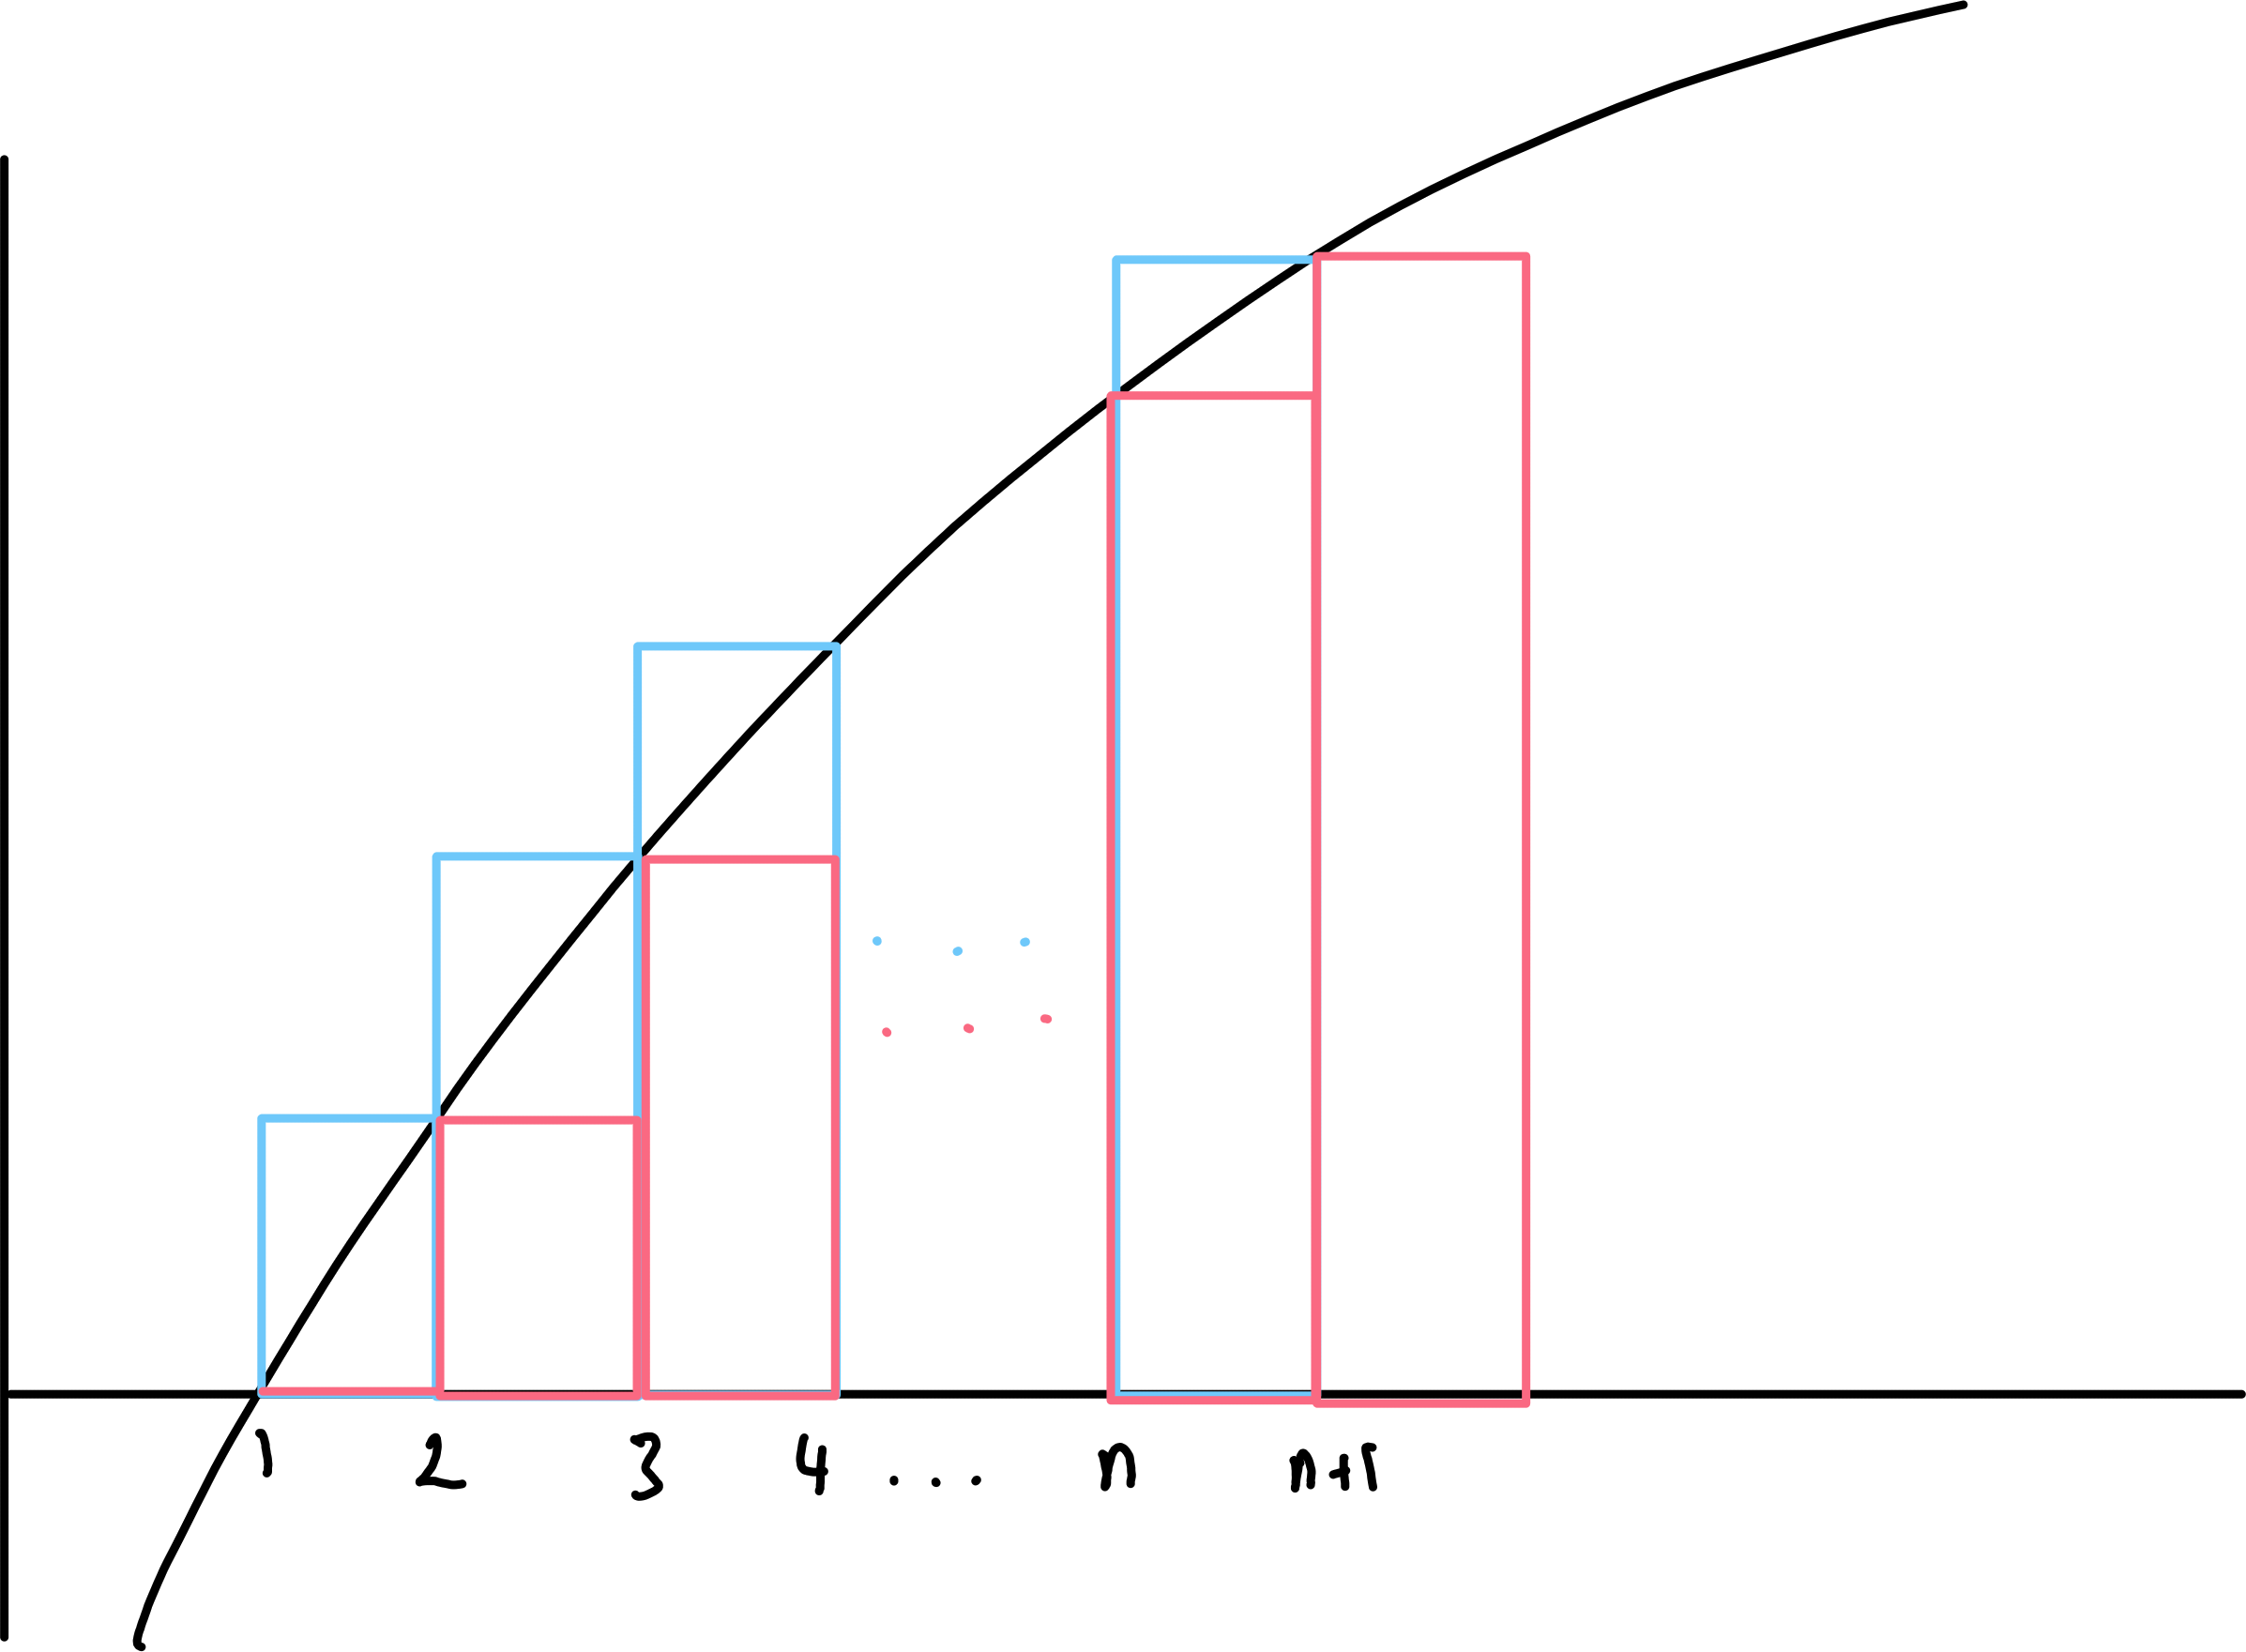
\includegraphics[height=5cm]{02-weak-1} \par}
    \begin{align*}
        \overset{``\text{Upper Integral}"}{\mathcolor{blue}{\int_{1}^{n} \log x \,dx}} \leq \log n! &\leq \overset{``\text{Lower Integral}"}{\mathcolor{red}{\int_{1}^{n + 1} \log x \,dx}} \\
        \underbrace{n \log n - n + 1}_{\sim n \log n} \leq \log n! &\leq \underbrace{(n + 1)\log(n+1) - n}_{\sim n \log n}
    \end{align*} 
    \emph{Key idea}: \emph{Sandwiching} between lower/upper integrals. It was useful that
    \begin{itemize}
        \item $\log x$ is increasing
        \item $\log x$ has a nice integral!
    \end{itemize} 
\end{proof}

\subsection{(Ordered) compositions} \label{Ordered compositions}

\begin{definition}[Composition]
    A \vocab{composition} of $m$ with $k$ parts is a sequence $(m_1, \dots, m_k)$ of non-negative integers with $m_1 + \dots + m_k = m$.
\end{definition} 
\begin{example}
    \begin{align*}
        &3 + 0 + 1 + 2 = 6 \color{red} \neq 1 + 2 + 0 + 3 = 6 \\
        &\star \star \star | | \star | \star \star
    \end{align*} 
\end{example} 

There is a bijection between compositions \emph{and} sequences of $m$ stars and $(k - 1)$ dividers.
So the number of compositions is $\binom{m + k -1}{m}$.

\emph{Comment:} Easy to mistake $k$ with $k - 1$ in no. of dividers.